% !TEX TS-program = xelatex
% !TEX encoding = UTF-8 Unicode

% Baseado no tutorial por Oliver Piters em lime_cv
% https://olivierpieters.be/blog/2017/09/12/designing-a-cv-in-latex-part-1


\documentclass[11pt]{article}

% hyphenation 
\usepackage[portuguese]{babel}
%\usepackage[british]{babel}

% more advanced expressions in \setlength
\usepackage{calc}

% force usage of newer commands (optinonal) 
\usepackage[l2tabu,orthodox]{nag}

% define margin
\newlength\cvMargin
\setlength\cvMargin{1cm}

\usepackage[margin=\cvMargin,noheadfoot,a4paper]{geometry}

% other lengths
\newlength\cvSideWidth
\setlength\cvSideWidth{0.3\paperwidth-\cvMargin}

\newlength\cvMainWidth
\setlength\cvMainWidth{\paperwidth-4\cvMargin-\cvSideWidth}

\newlength\cvPictureWidth
\setlength\cvPictureWidth{4cm}

\newlength\cvLanguageBarWidth
\setlength\cvLanguageBarWidth{5em}

\newlength\cvLanguageBarHeight
\setlength\cvLanguageBarHeight{0.75em}

\newlength\cvTimeDotSep
\setlength\cvTimeDotSep{0.4cm}

\newlength{\cvSectionSep}
\setlength{\cvSectionSep}{0.4cm}

\usepackage{calc}
\newlength\cvHeaderIconWidth

\newcommand{\cvSection}[1]{\Large\textbf{#1}}

\newcommand{\cvEducation}[4]{{\firaMedium #1}\\ \textsc{\selectfont #2} \\ {\color{cvdate_blue}#3} \\ \smallskip \emph{#4}}
\newcommand{\cvExperience}[5]{{\firaMedium #1}\\ \textsc{\selectfont #2} \\ \textsc{\selectfont #3} \\ {\color{cvdate_blue}#4}\\ \smallskip \emph{#5}}
\newcommand{\cvCertificate}[2]{{\firaMedium #1} \\ \smallskip \emph{#2}}


% links
\usepackage{hyperref}

% more advanced command definitions
\usepackage{xparse}

% advanced drawing
\usepackage{tikz}
\usetikzlibrary{calc,positioning,backgrounds,matrix,node-families}

% pictures
\usepackage{graphicx}

% define four main colours
\definecolor{cvDark}{HTML}{4a4a4a}
\definecolor{cvLight}{HTML}{beccd1}
\definecolor{cvGlobal}{HTML}{2F3142}
\definecolor{cvAccent}{HTML}{474A65}
\definecolor{cvdate_blue}{HTML}{045f8c}

% load external fonts
\usepackage{fontspec}    

% icon font
\usepackage{fontawesome}

% load external fonts
\setmainfont[Numbers={OldStyle,Monospaced}]{Fira Sans}
\setsansfont{Fira Sans}
\setmonofont{Fira Mono}
\newfontfamily\firaMedium{Fira Sans Medium}

\pagestyle{empty}

% update default paragraph indent, and header space
\setlength{\topskip}{0pt}      % between header and text (0 needed for vertical centring)
\usepackage{parskip}           % remove paragraph indents

% we can only set this length after loading the fonts
\setlength{\cvHeaderIconWidth}{\maxof{\widthof{\faBriefcase}}{\widthof{\faGraduationCap}}}

% set TikZ styles
\tikzset{
	contactIcon/.style={%
		minimum height=\baselineskip,
	},
	contactText/.style={%
		minimum height=\baselineskip,
		text depth=0pt,
	},
	headerIcon/.style={
		minimum width=\cvHeaderIconWidth,
		anchor=center,
	},
	languageText/.style={},
	progressArea/.style={%
		draw,
		rectangle,
		minimum width=\cvLanguageBarWidth,
		minimum height=\cvLanguageBarHeight,
		cvDark},
	progressBar/.style={%
		minimum height=\cvLanguageBarHeight,
		rectangle,
		draw,
		fill,
		cvDark,
		anchor=west},
	sectionTitle/.style={
		anchor=north west,
		align=left},
	eventdottext/.style = {
		text width=\cvMainWidth-\cvTimeDotSep,
		black,
		%text depth=0pt,
		anchor=north west,
	},
	sectionedutext/.style={
		eventdottext,
		anchor=north west
	},
	invisibletimedot/.style = {
		circle,
		minimum width=3pt,
		anchor=center
	},
	timedot/.style = {
		invisibletimedot,
		draw,
		minimum width=3pt,
		fill,
		black,
	},
}

% based on https://tex.stackexchange.com/questions/65731
\makeatletter
\def\cv@hrulefill{{\color{cvDark}\leavevmode\leaders\hrule height 1pt\hfill\kern\z@}}

% line before and after text (some tweaking is required here)
% based on https://tex.stackexchange.com/questions/15119
\NewDocumentCommand{\ruleline}{m}{\par\noindent\raisebox{\baselineskip/4}{\makebox[\linewidth]{\cv@hrulefill\hspace{1ex}\raisebox{-\baselineskip/4}{#1}\hspace{1ex}\cv@hrulefill}}}
\makeatother

% update global colour
\makeatletter
\NewDocumentCommand{\globalcolor}{m}{%
	\color{#1}\global\let\default@color\current@color
}
\makeatother
\AtBeginDocument{\globalcolor{cvGlobal}}

\NewDocumentCommand{\cvLanguage}{mm}{%
	{\globaldefs=1\relax\pgfkeys{/cv/languages/lang\the\value{languages} = #2}}
	
	\stepcounter{languages}
}

\makeatletter
\newcount\my@repeat@count
\newcommand{\cvSkill}[1]{%
	\begingroup
	\my@repeat@count=\z@
	\@whilenum\my@repeat@count<#1\do{\faCircle\advance\my@repeat@count\@ne}%
	\my@repeat@count=\numexpr5-\z@\relax
	\@whilenum\my@repeat@count>#1\do{\faCircleO\advance\my@repeat@count\m@ne}%
	\endgroup
}
\makeatother

\begin{document}
	
	\vspace*{\fill}
	\begin{tikzpicture}[remember picture,overlay]
	\fill[cvLight] (current page.north west) rectangle ++(\cvSideWidth+2\cvMargin,-\paperheight);
	\end{tikzpicture}
	\begin{minipage}{\cvSideWidth}
		\begin{center}
			
			\begin{tikzpicture}
			\node[
			circle,
			minimum size=\cvPictureWidth,
			path picture={
				\node at (path picture bounding box.center){
					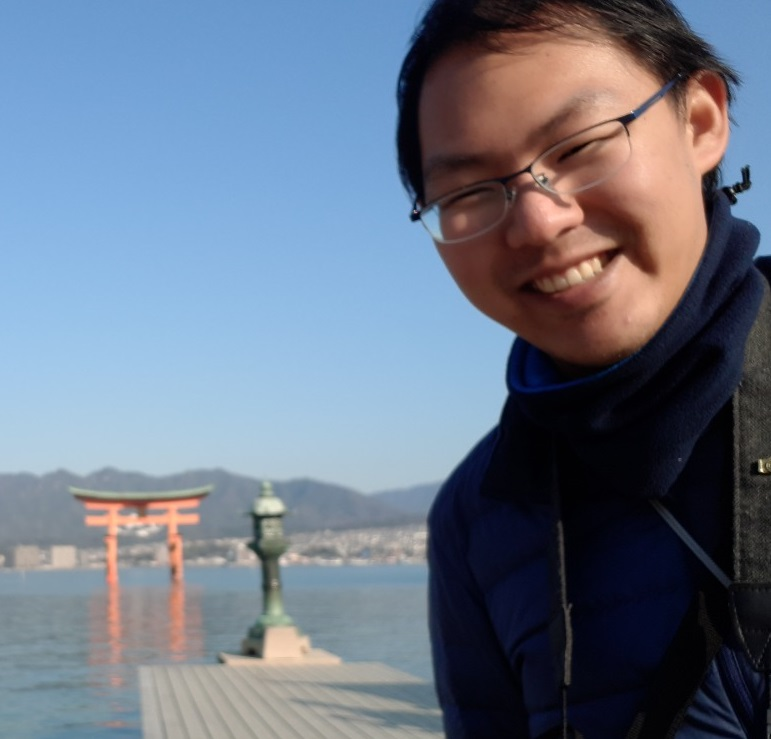
\includegraphics[width=\cvPictureWidth]{images/profile_picture.JPG}
				};
			}]
			{};
			\end{tikzpicture}
			
			{\LARGE
				Cesar Wen}
			
			{\color{cvAccent} 24 Anos}
			\vspace{0.5cm}
			
			
			
			{\color{cvAccent} Estudante de Engenharia Mecatrônica}
			
			\vspace{0.5cm}
			
			\ruleline{Perfil}
			
			Entusiasta por tecnologia, gosto de aprender e implementar novas tecnologias e ideias. Minha formação em engenharia mecatrônica permite a exploração e implementação de diversos produtos. \\Em meu tempo livre, gosto de realizar pequenos projetos pessoais.
			
			\vspace{4pt}
			
			\ruleline{Contato}
			
			\vspace{4pt}
			
			\begin{tikzpicture}[every node/.style={inner sep=0pt, outer sep=0pt}]
			\matrix [
			column 1/.style={anchor=center,contactIcon},
			column 2/.style={anchor=west,align=left,contactIcon},
			column sep=5pt,
			row sep=5pt] (contact) {
				\node{\faMapMarker}; 
				& \node{Brasil, São Paulo, SP\\Rua Verbo Divino, 1061};\\
				\node{\faEnvelope}; 
				& \node{\href{mailto:cesar.wen@usp.br}{cesar.wen@usp.br}};\\
				\node{\faPhone}; 
				& \node{+55 11 98706-4560};\\
				\node{\faWhatsapp}; 
				& \node{+81 80 2185-8005};\\
			%	\node{\faGlobe}; 
			%	& \node{\href{https://johndoe.com}{johndoe.com}};\\
				\node{\faGithub}; 
				& \node{\href{https://github.com/cesarwen}{cesarwen}};\\
				\node{\faLinkedinSquare}; 
				& \node{\href{https://www.linkedin.com/in/johndoe/}{cesarwen}};\\
			};
			\end{tikzpicture}
			
			\vspace{4pt}
			
			\ruleline{Línguas}
			
			\vspace{4pt}
			
			\begin{tikzpicture}[every node/.style={text depth=0pt,inner sep=0pt,outer sep=0pt}]
			\matrix [
			column 1/.style={anchor=east},
			column 2/.style={anchor=west},
			column sep=5pt,
			row sep=5pt,
			] (contact) {
				\node[languageText]{Portugês}; & \node[progressArea] (language 1) {}; \\
				\node[languageText]{Inglês};   & \node[progressArea] (language 2) {}; \\
				\node[languageText]{Espanhol}; & \node[progressArea] (language 3) {}; \\
				\node[languageText]{Chinês};   & \node[progressArea] (language 4) {}; \\
				\node[languageText]{Japonês};  & \node[progressArea] (language 5) {}; \\
				};
			\draw (language 1.west) node[progressBar,minimum width=5/5*\cvLanguageBarWidth] {};
			\draw (language 2.west) node[progressBar,minimum width=5/5*\cvLanguageBarWidth] {};
			\draw (language 3.west) node[progressBar,minimum width=4/5*\cvLanguageBarWidth] {};
			\draw (language 4.west) node[progressBar,minimum width=2/5*\cvLanguageBarWidth] {};
			\draw (language 5.west) node[progressBar,minimum width=1/5*\cvLanguageBarWidth] {};
			\end{tikzpicture}
			
			
			\vspace{5cm}
			\today
			
		\end{center}
	\end{minipage}
	\vspace*{\fill}
	
	
		%%%%%%%%%%%%%%
		% Main Page  %
		%%%%%%%%%%%%%%
	
	
	\begin{tikzpicture}[
	every node/.style={
		inner sep=0pt,
		outer sep=0pt
	},
	remember picture,
	overlay,
	shift={($(current page.north west)%
		+(\cvSideWidth+3\cvMargin+\cvTimeDotSep,-\cvMargin)$)}]
	% main content  
	
	\node[sectionTitle] at (0,0) (title 1) {\cvSection{Educação}};
	\node[left=\cvTimeDotSep of title 1,headerIcon] {\faGraduationCap};
	\begin{scope}[on background layer]
	\draw[line width=2pt,cvDark] 
	let \p1=(title 1.south west), 
	\p2=(current page.east) in 
	(\x1,\y1-0.1cm) to (\x2,\y1-0.1cm);
	\end{scope}
	
	% item 1
	\node[
	below=\cvSectionSep of title 1.south west,
	eventdottext] 
	(item 1 header) 
	{\phantom{Graduação}};
	\node[
	below=\cvSectionSep of title 1.south west,
	sectionedutext] 
	(item 1) 
	{\cvEducation{Graduação em Engenharia Mecatrônica}%
		{Escola Politécnica da Universidade de São Paulo}
		{2015 -- Presente}%
		{Estudos de sistemas mecânicos, eletrônicos, computacionais e de controle.}};
	\node[
	left=\cvTimeDotSep of item 1 header,
	timedot] 
	(start) 
	{};
	
	% item 2
	\node[
	below=\cvSectionSep of item 1.south west,
	eventdottext] 
	(item 2 header) 
	{\phantom{Intercâmbio}};
	\node[
	below=\cvSectionSep of item 1.south west,
	sectionedutext] 
	(item 2) 
	{\cvEducation{Intercâmbio}%
		{Shibaura Intitute of Technology, Saitama, Japão}
		{Agosto 2018 -- Agosto 2019}%
		{Estudos sobre robótica, mecatrônica e programação além da cultura e língua japonesa sob o programa "Sandwich Program" oferecido pela faculdade no exterior em parceria com a Escola Politécnica.}};
	\node[
	left=\cvTimeDotSep of item 2 header,
	timedot] 
	{};
	
	% item 3
	\node[
	below=\cvSectionSep of item 2.south west,
	eventdottext] 
	(item 3 header) 
	{\phantom{Evening}};
	\node[
	below=\cvSectionSep of item 2.south west,
	sectionedutext] 
	(item 3) 
	{\cvEducation{Ensino Médio}%
		{Colégio Bandeirantes}
		{Janeiro 2010 -- Dezembro 2013}%
		{Estudos sobre conteúdos gerais e multiplas oportunidadeds de estudos em diversos temas como aulas de espanhol e oficina mecatrônica.}};
	\node[
	left=\cvTimeDotSep of item 3 header,
	timedot] 
	{};
	
	\node[
	left=\cvTimeDotSep of item 3.south west,
	invisibletimedot] 
	(end) 
	{};
	\draw (start) to (end.center);
	
	%%%%%%%%%%%%%%
	% Experience %
	%%%%%%%%%%%%%%
	
	\node[below=0.6cm of item 3.south west,sectionTitle] (title 2) {\cvSection{Atividades Extracurriculares}};
	\node[left=\cvTimeDotSep of title 2,headerIcon] {\faNewspaperO};
	\node[below=0.6cm of item 3.south west,sectionTitle] (title 2 dummy) {\phantom{\cvSection{Educação}}};
	\begin{scope}[on background layer]
	\draw[line width=2pt,cvDark] 
	let \p1=(title 2 dummy.south west), 
	\p2=(current page.east) in 
	(\x1,\y1-0.1cm) to (\x2,\y1-0.1cm);
	\end{scope}
	
	\node[
	below=\cvSectionSep of title 2.south west,
	eventdottext] 
	(item 1 header) 
	{\phantom{Evening}};
	\node[
	below=\cvSectionSep of title 2.south west,
	sectionedutext] 
	(item 1) 
	{\cvExperience%
		{Iniciação Científica}%
		{Laboratório de Percepção Avançada (LPA)}%
		{Escola Politécnica da USP}%
		{Fevereiro 2017 -- Fevereiro 2018}%
		{Software de aquisição de dados de estações meteorológicas para a análise de conforto ambiental.}};
	\node[
	left=\cvTimeDotSep of item 1 header,
	timedot] 
	(start) 
	{};
	
	% item 2
	\node[
	below=\cvSectionSep of item 1.south west,
	eventdottext] 
	(item 2 header) 
	{\phantom{Evening}};
	\node[
	below=\cvSectionSep of item 1.south west,
	sectionedutext] 
	(item 2) 
	{\cvExperience%
		{Projeto}%
		{Arquiteturas de Base Reconfiguráveis (ABRA)}%
		{Escola Politécnica da USP}%
		{Março 2019 -- Agosto 2018}%
		{Construção e melhoria de impressoras 3D baseadas em tecnologia de fusão (FDM).}};
	\node[
	left=\cvTimeDotSep of item 2 header,
	timedot] 
	{};
	

	\node[
	left=\cvTimeDotSep of item 2.south west,
	invisibletimedot] 
	(end) 
	{};
	\draw (start) to (end.center);
	
	%%%%%%%%%%
	% Skills %
	%%%%%%%%%%
	
	\node[below=0.6cm of item 2.south west,sectionTitle] (title 3) {\cvSection{Programação}};
	\node[left=\cvTimeDotSep of title 3,headerIcon] {\faFileCodeO};
	\node[below=0.6cm of item 2.south west,sectionTitle] (title 3 dummy) {\phantom{\cvSection{Educação}}};
	\begin{scope}[on background layer]
	\draw[line width=2pt,cvDark] 
	let \p1=(title 3 dummy.south west), 
	\p2=(current page.east) in 
	(\x1,\y1-0.1cm) to (\x2,\y1-0.1cm);
	\end{scope}
	
	\matrix[matrix of nodes,
	below=0.6cm of title 3.south west,
	anchor=north west,
	column sep=6pt,
	row sep=6pt,
	every node/.style={Text Depth=tdSkills},
	column 1/.style={anchor=east,align=left},
	column 2/.style={anchor=west},
	column 3/.style={anchor=east,align=left},
	column 4/.style={anchor=west},
	column 5/.style={anchor=east,align=left},
	column 6/.style={anchor=west}] (skills) {
		\cvSkill{4} & MATLAB\hspace{0.5cm}   & \cvSkill{2} & \LaTeX                & \cvSkill{4} & mySQL\\
		\cvSkill{4} & Python                 & \cvSkill{3} & Java\hspace{0.5cm}    & \cvSkill{3} & C, C++\\};	

	%%%%%%%%%%%%%%
	% Tools      %
	%%%%%%%%%%%%%%
	
	\node[below=0.6cm of skills.south west,sectionTitle] (title 4) {\cvSection{Ferramentas}};
	\node[left=\cvTimeDotSep of title 4,headerIcon] {\faCogs};
	\node[below=0.6cm of skills.south west,sectionTitle] (title 4 dummy) {\phantom{\cvSection{Educação}}};
	\begin{scope}[on background layer]
	\draw[line width=2pt,cvDark] 
	let \p1=(title 4 dummy.south west), 
	\p2=(current page.east) in 
	(\x1,\y1-0.1cm) to (\x2,\y1-0.1cm);
	\end{scope}
	
	
	\matrix[matrix of nodes,
	below=0.6cm of title 4.south west,
	anchor=north west,
	column sep=6pt,
	row sep=6pt,
	every node/.style={Text Depth=tdSkills},
	column 1/.style={anchor=east,align=left},
	column 2/.style={anchor=west},
	column 3/.style={anchor=east,align=left},
	column 4/.style={anchor=west},] (skills) {
		\cvSkill{3} & Fusion 360           				  & \cvSkill{4} & Visual Studio Code\\
		\cvSkill{3} & Autodesk Inventor\hspace{0.5cm}     & \cvSkill{3} & Pacote Office\\};
		
		
	%%%%%%%%%%%%%%%%
	% Certificates %
	%%%%%%%%%%%%%%%%	

	\node[below=0.6cm of skills.south west,sectionTitle] (title 5) {\cvSection{Certificados}};
	\node[left=\cvTimeDotSep of title 5,headerIcon] {\faCheckSquareO};
	\node[below=0.6cm of skills.south west,sectionTitle] (title 5 dummy) {\phantom{\cvSection{Educação}}};
	\begin{scope}[on background layer]
	\draw[line width=2pt,cvDark] 
	let \p1=(title 5 dummy.south west), 
	\p2=(current page.east) in 
	(\x1,\y1-0.1cm) to (\x2,\y1-0.1cm);
	\end{scope}

	\node[
	below=\cvSectionSep of title 5.south west,
	eventdottext] 
	(item 1 header) 
	{\phantom{Graduação}};
	\node[
	below=\cvSectionSep of title 5.south west,
	sectionedutext] 
	(item 1) 
	{\cvCertificate
		{TOEFL IBT - 101}
		{Um dos maiores certificados de inglês do  mundo. (Potuação máxima: 120)}};
	\node[
	left=\cvTimeDotSep of item 1 header,
	timedot] 
	(start) 
	{};
	
	\node[
	below=\cvSectionSep of item 1.south west,
	eventdottext] 
	(item 2 header) 
	{\phantom{Graduação}};
	\node[
	below=\cvSectionSep of item 1.south west,
	sectionedutext] 
	(item 2) 
	{\cvCertificate
		{Curso Avançado de Língua Espanhola e Cultura Hispânica}
		{Certificado do curso de espanhol oferecido pelo Colégio Bandeirantes. (Aprovado)}};
	\node[
	left=\cvTimeDotSep of item 2 header,
	timedot] 
	{};
	
	\node[
	left=\cvTimeDotSep of item 2.south west,
	invisibletimedot] 
	(end) 
	{};
	\draw (start) to (end.center);
		
	\end{tikzpicture}
	
\end{document}